
\begin{frame}{Literature Review}
    \begin{block}{how to kill a tracklet}
        Quite a lot teams are investigating the issue of when to die.
        \href{https://arxiv.org/pdf/2107.04327.pdf}{\beamergotobutton{preprint}}
        \begin{figure}
        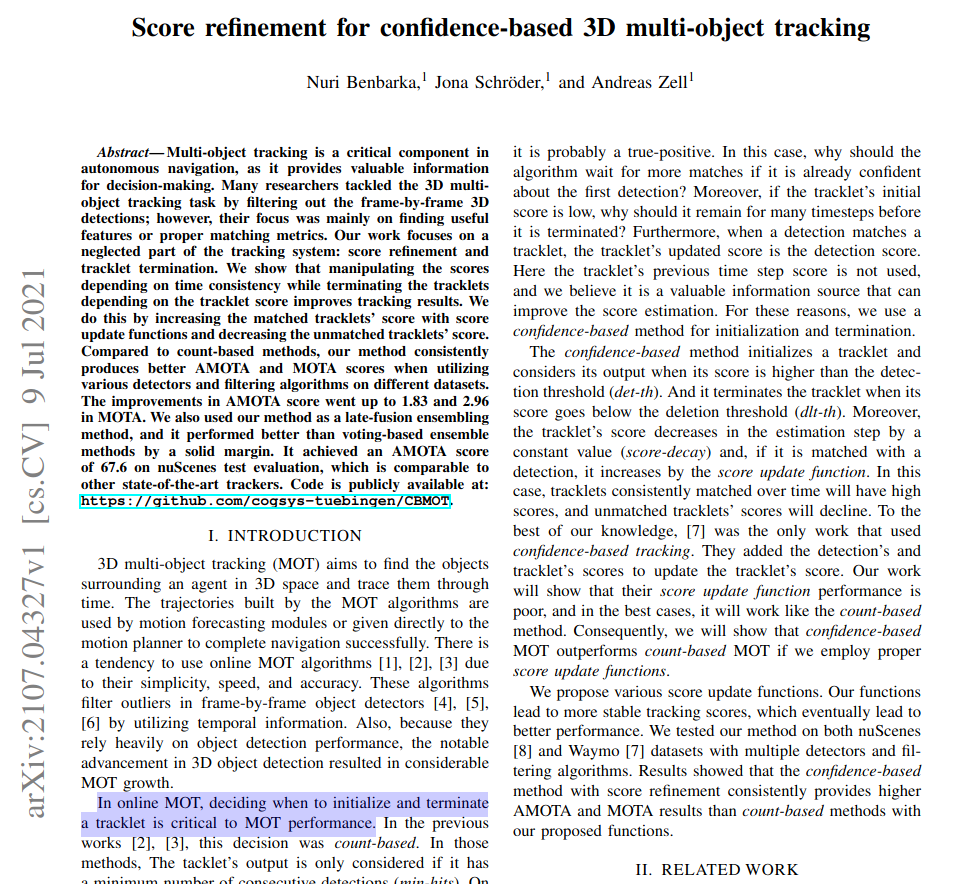
\includegraphics[width=0.4\linewidth]{termination/1.png}
        \end{figure}
    \end{block}
    \end{frame}
    
    \begin{frame}{Literature Review}
    \begin{block}{how to kill a tracklet}
        Case Study \href{https://arxiv.org/pdf/2111.13672.pdf}{\beamergotobutton{preprint}}
        \begin{figure}
        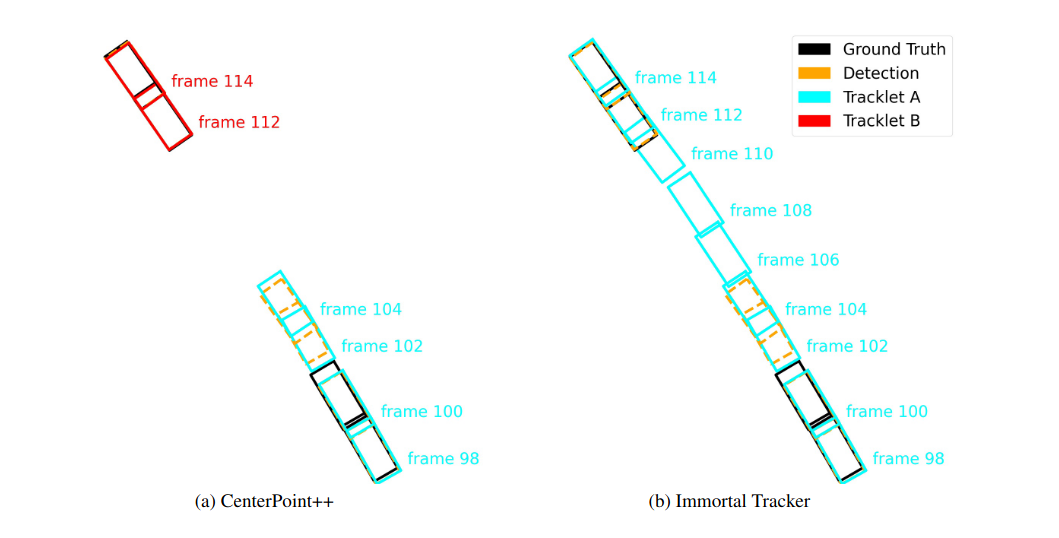
\includegraphics[width=0.9\linewidth]{termination/2.png}
        \end{figure}
    \end{block}
    \end{frame}
    
    \begin{frame}{PMBM adjustment}
        So unlike a standard PMBM filter, we incorporate the detection confidence score into the update step 
        of \textbf{objects detected for the first time}. 
        For detections with confidence scores larger than a threshold, 
        we generate a potential new target by adding \textbf{a new Bernoulli process}, 
        and plug the negative logarithm weight in the right m × m blocks diagonal in cost matrix L 
        discussed in Section IV-C. For detections with lower confidence score, 
        since we are not certain about their existences and require more evidences from the future, 
        an undetected track with PPP density is generated for each of them.
        \href{https://www.researchgate.net/publication/355428771_3D_Multi-Object_Tracking_using_Random_Finite_Set-based_Multiple_Measurement_Models_Filtering_RFS-M_3_for_Autonomous_Vehicles}{\beamergotobutton{paper}}
        
    \end{frame}
    
    \begin{frame}{PMBM adjustment}
        Add new Gaussian to the mixture (which represent the poisson intensity). This birth process is driven by
        measurements. Each measurement induce 3 birth of the same class by adding noise (uniformly distributed)
        \href{https://github.com/quan-dao/pmbm-filter/blob/5cdf8b31665f1a7008afa963c1ab7c3b048b5856/poisson.py}{\beamergotobutton{repository}}
    
        \begin{figure}
            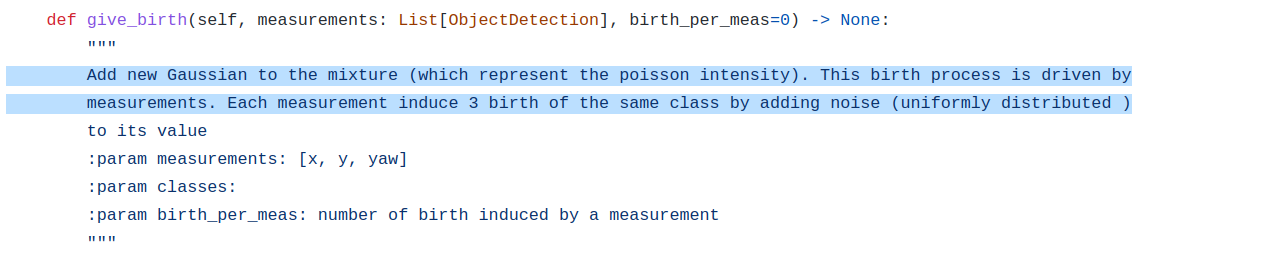
\includegraphics[width=0.9\linewidth]{pmbm/1.png}
        \end{figure}
    \end{frame}
    

\begin{frame}{Literature Review}
    \begin{block}{Measurement-Track association NOT a performance constraint for Lidar based MOT}
        \begin{figure}
        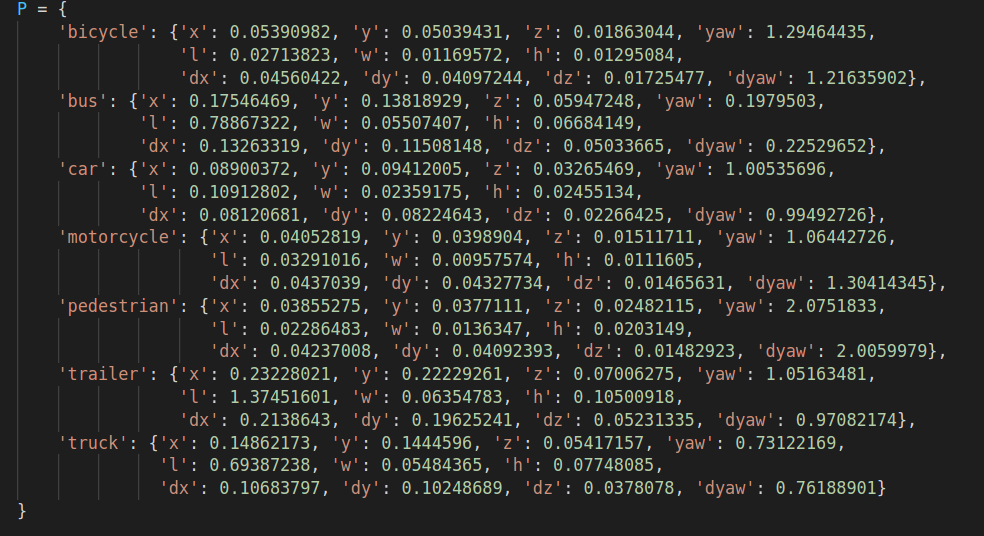
\includegraphics[width=0.9\linewidth]{DA/2.png}
        \end{figure}
    \end{block}
    \end{frame}
    
    \begin{frame}{Literature Review}
    \begin{block}{Measurement-Track association NOT a performance constraint for Lidar based MOT}
        \begin{figure}
        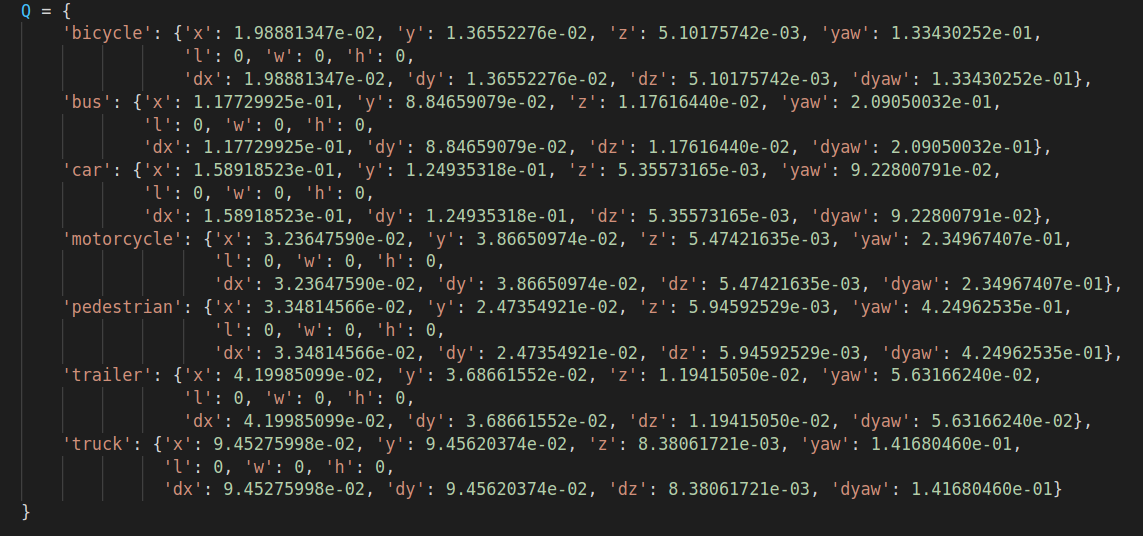
\includegraphics[width=0.9\linewidth]{DA/3.png}
        \end{figure}
    \end{block}
    \end{frame}
    
    \begin{frame}{Literature Review}
    \begin{block}{Measurement-Track association NOT a performance constraint for Lidar based MOT}
        \begin{figure}
        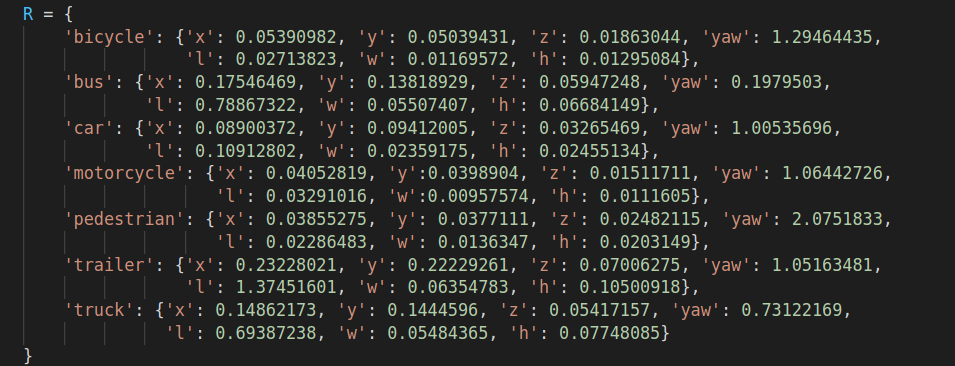
\includegraphics[width=0.9\linewidth]{DA/4.png}
        \end{figure}
    \end{block}
    \end{frame}
    
    
    
    \begin{frame}{RFS has a lot to contribute NOT in association but in track management}
        \begin{itemize}
            \item{how to strike a balance between Immortal track and Early Termination}
            \item{silent maintanance of the tracklet}
        \end{itemize}
    \end{frame}
    
    \begin{frame}{Incorporating Detection Score provided by the detector}
        \begin{itemize}
            \item{two stage association}
            \item{counters for the track}
        \end{itemize}
    \end{frame}